\documentclass[10pt,aspectratio=169]{beamer}

% All the boilerplate is in ccaslides.sty
% Note that this also pulls in a custom vogtwidebar.sty
\usepackage{ccaslides}

\author{Ji\v{r}\'i Lebl}

\institute[OSU]{%
Departemento pri Matematiko de Oklahoma {\^S}tata Universitato}

\title{Cultivating Complex Analysis:\\%
Automorphisms of the disc (3.5.2)}

\date{}

\begin{document}

\begin{frame}
\titlepage
\end{frame}

\begin{frame}
Recall, an automorphism of $U$ is a biholomorphism $f \colon U \to U$

(bijective such that $f$ and $f^{-1}$ are both holomorphic).

\medskip
\pause

Let us compute the automorphism group of the disc, $\Aut(\D)$.

\medskip
\pause

We start with certain specific automorphisms.

\medskip
\pause

For $a \in \D$, define
\[
\varphi_a(z) \overset{\text{def}}{=} \frac{z-a}{1-\bar{a}z}.
\]

\pause

\begin{proposition}
For every $a \in \D$,
\begin{enumerate}[(i)]
\item
$\varphi_a(a) = 0$, \enspace
$\varphi_a(0) = -a$, \enspace
$\varphi_a'(0) = 1 - \sabs{a}^2$, \enspace
$\varphi_a'(a) = \frac{1}{1 - \sabs{a}^2}$,
\pause
\item
$\varphi_a(\partial \D) = \partial \D$,
and
$\varphi_a(\D) = \D$,
\pause
\item
$\varphi_a$ restricted to $\D$ is an automorphism of the disc and
$\varphi_a^{-1} = \varphi_{-a}$.
\end{enumerate}
\end{proposition}
\pause

Proof is an exercise.
\end{frame}

\begin{frame}
Here is what an automorphism $\varphi_a$ does ($a=-0.4$).

\begin{center}
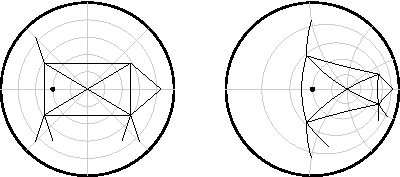
\includegraphics{../figures/varphiplot}
\end{center}

$a$ and $\varphi_a(a)=0$ are marked with dots.

\pause
\medskip

It turns out all automorphisms are $\varphi_a$ up to a rotation:

\pause

\begin{proposition}
If $f \in \Aut(\D)$, then there exists an $a \in \D$
and $\theta \in \R$ such that
\begin{equation*}
f(z) = e^{i\theta} \frac{z-a}{1-\bar{a}z} = e^{i\theta} \varphi_a(z).
\end{equation*}
\end{proposition}

\end{frame}

\begin{frame}
\textbf{Proof:}
Let $a = f(0)$.

\medskip
\pause

$g = \varphi_a \circ f$ is an automorphism with $g(0) = 0$ as
$\varphi_a(a) = 0$.

\medskip
\pause

Find a holomorphic $h(z)$ such that $g(z) = z h(z)$ (as in the proof of
Schwarz).

\medskip
\pause

Schwarz says that for $z \in \D \setminus \{ 0 \}$, \quad
$\sabs{h(z)} = \dfrac{\sabs{g(z)}}{\sabs{z}} \leq 1$.

\medskip
\pause

$h$ can have no zeros:
\pause
$h(z) = \frac{g(z)}{z}$ cannot be zero for $z \not= 0$ as $g$ is injective,

\pause
and it cannot have a zero at $z=0$
as $h(0) = \lim\limits_{z\to 0} \frac{g(z)}{z} = g'(0) \not= 0$.

\pause
\medskip

$g$ is biholomorphic
~ $\Rightarrow$ ~
$g^{-1}$ is continuous
\pause
~ $\Rightarrow$ ~
$g^{-1}(K)$ compact for compact $K \subset \D$

\medskip

\pause
$\Rightarrow$ ~
$\sabs{g(z)} \to 1$ as $\sabs{z} \to 1$ (exercise)
\pause
~ $\Rightarrow$ ~
$\sabs{h(z)} \to 1$ as $\sabs{z} \to 1$

\medskip
\pause

$\Rightarrow$ ~
$\sabs{h(z)}$ attains a minimum in $\D$
\pause
~ $\Rightarrow$ ~
$\babs{\frac{1}{h(z)}}$ attains a maximum in $\D$
\pause
~ $\Rightarrow$ ~
$h$ is constant

\medskip
\pause

$\Rightarrow$ ~
$g(z) = \alpha z$ for some constant $\alpha$.
\pause
As $g \in \Aut(\D)$, ~
$\sabs{\alpha} = 1$ ~ ($\alpha = e^{i\theta}$).

\medskip
\pause

Apply $\varphi_{-a}$ to both sides of $e^{i\theta} z = \varphi_a \circ f$
to find
$f(z) = \varphi_{-a}(ze^{i\theta})
= e^{i \theta} \varphi_{-ae^{-i\theta}}(z)$.
\qed

\end{frame}

\begin{frame}

Some good exercises to try:

\medskip

\textbf{Exercise:}
Given distinct $a,b \in \D$, show that there exists a unique 
$f \in \Aut(\D)$
such that $f(a) = b$ and $f(b) = a$.

\pause
\medskip

\textbf{Exercise:}
The automorphisms of $\bH = \{ z \in \C : \Im z > 0 \}$
are of the form
$\frac{a z +b}{c z + d}$
for real numbers $a,b,c,d$ such that $ad-bc \not= 0$.

\pause
\medskip

Another fun exercise, a version of which seems to appear on many exams is
the following:

\medskip
\textbf{Exercise:}
Suppose $U \subset \C$ is a domain, $\overline{\D} \subset U$,
and $f \colon U \to \C$ is holomorphic such that
$f(\partial \D) \subset \partial \D$.
Find a formula for $f$.

\medskip
\pause

Hint: 
The idea is to show that you can divide by finitely many
$\varphi_a(z)$ for various $a$ until you get something that has no zeros in
$\D$ and will have to be a constant.

\end{frame}

\begin{frame}
Using automorphisms one proves an ``invariant version'' of the Schwarz lemma.

\pause

\begin{lemma}[Schwarz--Pick]
If $f \colon \D \to \D$ is holomorphic, then
\begin{equation*}
\abs{
\frac{f(z)-f(\zeta)}{1-\overline{f(\zeta)}f(z)}
}
\leq
\abs{
\frac{z-\zeta}{1-\widebar{\zeta}z} 
}
\qquad
\text{and}
\qquad
\frac{\abs{f'(z)}}{1-\abs{f(z)}^2} \leq
\frac{1}{1-\abs{z}^2}
\qquad
\text{for all } z,\zeta \in \D.
\end{equation*}
\pause
If equality holds in one of the 
inequalities for some $z \not= \zeta$,
then $f \in \Aut(\D)$.
\pause

Conversely, if $f \in \Aut(\D)$,
then equality holds in both inequalities for
all $z,\zeta \in \D$.
\end{lemma}

\pause

Proof is an exercise.

\medskip
\pause


The Schwarz--Pick lemma gives a bound on the derivative
at all points:

If $f \colon \D \to \D$ is holomorphic, nonconstant, and $f(a) = b$,
then
\[
\sabs{f'(a)} \leq
\frac{1-\sabs{b}^2}{1-\sabs{a}^2} .
\]
\pause
Equality $\Rightarrow$ $f(z) = \varphi_{-b}\bigl( e^{i\theta} \varphi_a(z)
\bigr)$ for some $\theta \in \R$.
\end{frame}

\end{document}
